\documentclass[master.tex]{subfiles}

\begin{document}

\section*{C. Approach}

\subsection*{Aim 1: Study the effect of emotional value on the extent and symmetry
  of the temporal window of memory linking.}

\begin{figure}[!b]
\centering
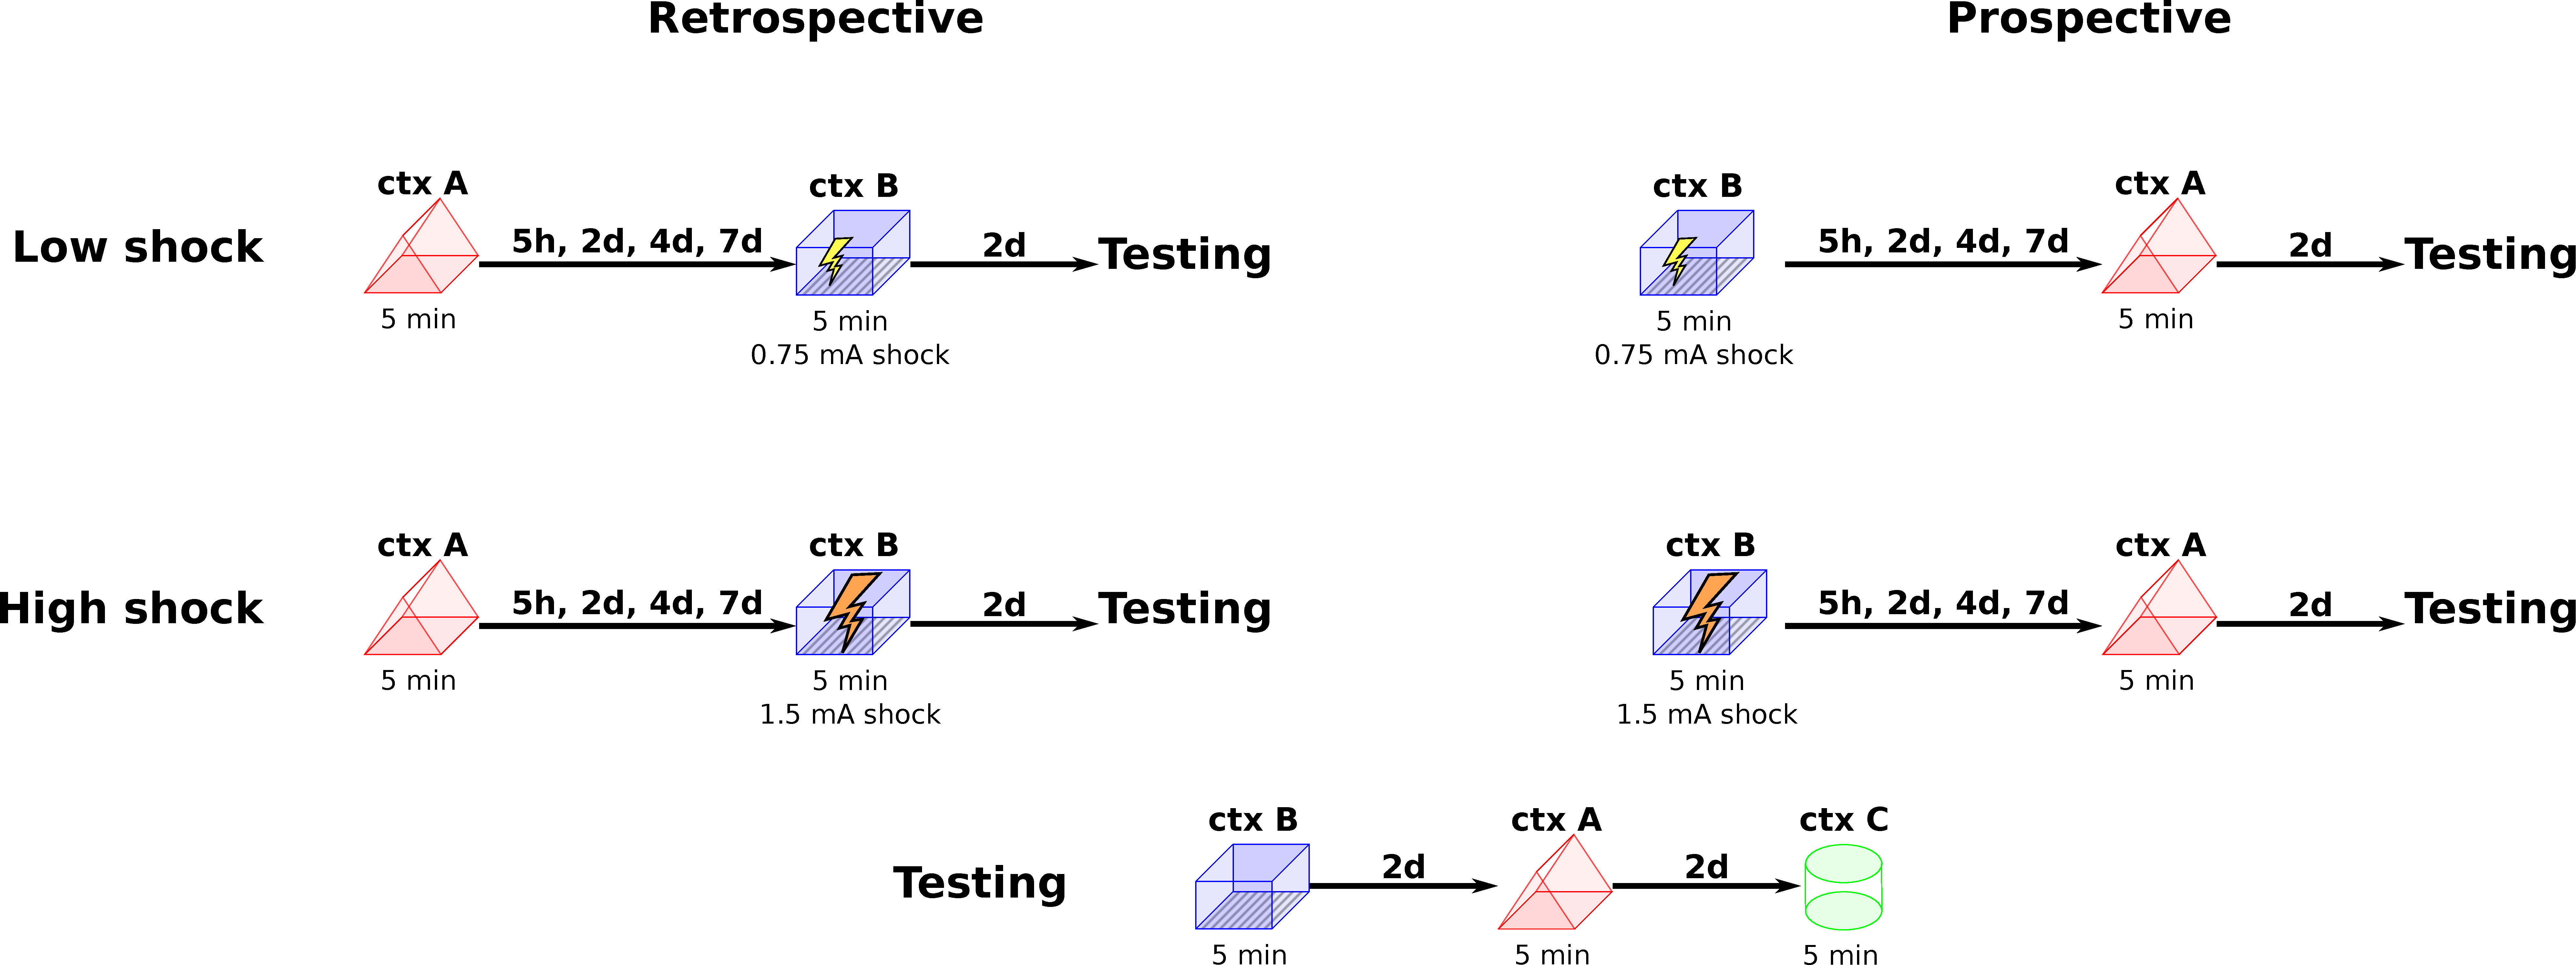
\includegraphics[scale = .135]{Figures/full.pdf}
\caption{\footnotesize behavior experimental design}
\label{fig1}
\end{figure}

To test the hypothesis, we will use contextual fear conditioning combined with
calcium imaging in behaving mice. We choose contextual fear conditioning because
it is a robust and well-established test for long-term memory, and moreover a
strong memory can be formed within one learning session. We choose miniature
calcium imaging due to its capability to record neuronal activities in behaving
mice and to track same field-of-view across long period of time, which is
essential for the purpose of memory linking studies. We will focus on recording
in dorsal CA1 region since it is believed to make a major contribution to
contextual memory.

The presented proposal will adopt a similar experimental design. Specifically,
animals will be divided into two groups: ``neutral'' and ``negative'', which
represent the affective value of the shocking context during encoding. Both
groups will explore context A, B and C for 10 minutes. The time point at which
the animals experience A, B and C is spaced out in such a way that the temporal
distances between each of them and the shocking context S is 7 days, 2 days and
5 hours respectively. During the exploration of the shocking context S, a 2
seconds long, 0.1 mA delayed shock will be delivered at fifth minute to the
animals in ``negative'' group, but not ``neutral'' group. Both groups explore
the shocking context S for 10 minutes. Then 2 days later, animals in the
``neutral'' group will be put back in context S, where a 2 seconds long, 0.1 mA
immediate shock is delivered after 10 seconds of exploration. Finally, another 2
days later (that is, 4 days interval for ``negative group''), each group of
animals are further divided into 5 sub-groups, where their freezing levels are
assessed in parallel for context A, B, C, S, as well as N, which is a novel
context. Neuronal activities in dorsal CA1 are recorded with miniature
endoscope throughout the whole experiment.

We expect to see significantly higher freezing levels in context B, C, and S
when comparing to A or N in ``negative'' group, while only freezing levels in C
and S are significantly higher when comparing to either A, N or C in ``neutral''
group. Furthermore, we expect in ``negative'' group that the overlap of neural
ensembles between B and S, as well as between C and S, are significantly higher
than the overlaps between A and S or N and S, which is supposedly at ``chance''
level. Whereas in ``neutral'' group, the overlaps between A and S, B and S, as
well as N and S should all be low and at ``chance'' level, while only the
overlaps between C and S are significantly higher than others. Taken together,
these results would suggest that the paring of context S with shock during
encoding extend the time window of memory linking to at least 2 days back, while
the memory linking time window for a neutral context is only longer than 5 hours
but shorter than 2 days.


\subsection*{Aim 2: Test the hypothesis that prospective memory linking has a
  different temporal window comparing to retrospective memory linking.}

Similar to Aim 1, we use contextual fear conditioning combined with calcium
imaging to test the hypothesis.


The presented proposal use a similar setup. Specifically, animals are divided
into two groups, ``prospective'' and ``retrospective''. The animals in
``retrospective'' group will explore context A, B and C before the shocking
context S, while those in ``prospective'' group will explore A, B and C after
the shocking context S. The time points at which the animals explore A, B and C
are spaced out such that the temporal distance between the shocking context S
and context A, B or C are 2 days, 1 day and 5 hours respectively. In both
groups, animals explore context A, B, C, S for 10 minutes, where during
exploration of context S, a 2 seconds, 0.1 mA shock will be delivered at the
fifth minute. 2 days after the exploration are finished for the last context,
each group will be further divided into 5 sub-groups, where their freezing
levels are assessed in parallel in context A, B, C, S, as well as N, which is a
novel context. Neuronal activities in dorsal CA1 are recorded with miniature
endoscope throughout the whole experiment.

We expect to see elevated freezing level for context B, C and S comparing to A
and N in ``retrospective'' group, whereas in ``prospective'' group freezing
levels are only higher in C and S, but not A, B or N. Furthermore, we expect the
overlap in ensembles between B and S as well as between C and S are higher in
``retrospective'' group, whereas in ``prospective'' group the overlap are only
higher between C and S but not between B and S, when comparing to the ``chance''
level overlap between N and S. Taken together, these results would suggest that
``prospective'' memory linking has a shorter temporal window than
``retrospective'' temporal linking.

\subsection*{Aim 3: Test the hypothesis that linked memories have higher
  similarity of ensemble structures.}
The raw videos from calcium imaging recording could be processed with an
open-source analysis toolkit CaImAn implementing a constrained non-negative
matrix factorization algorithm. After the process, a spatial matrix representing
the spatial footprint of each putative neurons, as well as a temporal matrix
representing the calcium traces of each putative neurons will be extracted from
the raw data. A custom-written script is used to visually assess the accuracy of
the extraction as well as manually refine the results. After this, neurons from
different recording sessions are cross-registered based on the euclidean
distances between the centroids of their spatial footprint, and a unique master
index can be assigned to each neuron in the whole experiment.

For each recording session, given a matrix representing the calcium traces of
$N$ neurons along $T$ time-steps (usually frames), a PCA analysis can be applied
to extract $R$ principal components, where each components contain a ``neuron
vector'' $\vec{n}$ of length $N$, and a ``temporal vector'' $\vec{t}$ of length
$T$. Thus the dimension of the data is reduced from $N \times T$ to $R \times (N
+ T)$. The PCA is carried out in a way so that:
\begin{inparaenum}[a)]
\item the ``neuron vector'' of each principle component represent a group of
  neurons that has a highly correlated firing pattern, and the ``temporal
  vector'' represent that averaged pattern treating the whole group as single
  neuron.
\item a dot product can be computed with each ``neuron vector'' and ``temporal
  vector'', and the sum of $R$ such dot products should closely reproduce the
  original $N \times T$ data.
\item the $R$ components should explain most of the variance in the original
  data, thus the value of $R$ can be determined by thresholding the proportion
  of variance explained.
\end{inparaenum}

Once the principal components of each recording sessions are extracted, we can
calculate a cross-correlation of the ``neuron vector''s between any two session.
We can then compare such correlation matrices between linked context and
unlinked contexts. We expect to see higher correlations between linked contexts,
suggesting that the temporally correlated structures within each ensemble are
more likely to be preserved across linked contexts than across unlinked
contexts.

The presented approach has two caveats that might require further refining:
Firstly, a method to assess the quality of cross-registration is lacking. For
this issue, an algorithm developed by Yaniv lab might be more suitable since it
can also output the confidence of cross-registration. However, as long as the
current approach does not produce systematic bias towards linked contexts, that
is, as long as the field-of-view of recordings remain relatively stable, there
is no reason to expect a significant artifact from presented methods. Secondly,
the application of PCA analysis presume that the neuronal ensembles are
structured such that subsets of cells fire together. It may fail to detect other
temporal structures, such as sequence of firing. For this, other dimension
reduction algorithms might address the issue.
\end{document}